% SC2002 --- Chapter 2: Classes & Encapsulation (0->100 ground-up)
\chapter{Classes \& Encapsulation: From Objects to Blueprints}
\label{ch:classes}

\begin{quote}
\emph{``A class is a cookie cutter; objects are the cookies.''} --- One object is an example; a \emph{class} is the recipe. Encapsulation decides what the recipe reveals and what it hides. This chapter turns the object intuition from Ch.~1 into code-level discipline.
\end{quote}

\noindent\fbox{\parbox{\dimexpr\linewidth-2\fboxsep-2\fboxrule}{%
\textbf{From zero: built on Ch.~1 only.} We define \emph{class}, \emph{field}, \emph{method}, \emph{constructor}, and \emph{visibility} from scratch. Java is our notation but the ideas port to C\#, Python, C++. No prior Java assumed.}}
\vspace{0.4em}

\section*{Learning Outcomes}
After this chapter you will be able to:
\begin{enumerate}[label=(L\arabic*)]
    \item distinguish \emph{class} (type/blueprint) from \emph{object} (instance) and explain instantiation;
    \item declare fields, constructors, accessors/mutators, and enforce invariants via encapsulation;
    \item apply access modifiers (\texttt{private}, package, \texttt{protected}, \texttt{public}) and \texttt{static} vs.\ instance;
    \item reason about object identity vs.\ equality (\texttt{==} vs.\ \texttt{equals}) and \texttt{toString} contracts;
    \item justify information hiding using coupling and change-impact arguments.
\end{enumerate}

% ============================================================
\section{Classes as Blueprints}
\label{sec:blueprints}
In Ch.~1 an \emph{object} was identity + state + behaviour. A \emph{class} packages the shared structure for many such objects: it declares what fields every instance has, what methods it offers, and how instances are created.

\begin{figure}[h]
\centering
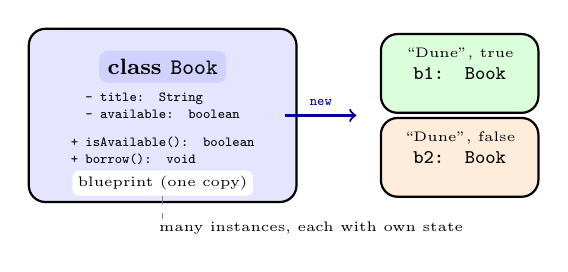
\begin{tikzpicture}[scale=0.82, every node/.style={font=\scriptsize}]
\node[draw,thick,fill=blue!10,rounded corners=6pt,minimum width=3.4cm,minimum height=2.2cm] (cls) at (0,0) {};
\node[font=\footnotesize\bfseries,fill=blue!18,rounded corners=3pt,inner sep=3pt] at (0,0.75) {class \texttt{Book}};
\node[font=\tiny,align=left] at (0,0.15) {\texttt{- title: String}\\\texttt{- available: boolean}};
\node[font=\tiny,align=left] at (0,-0.55) {\texttt{+ isAvailable(): boolean}\\\texttt{+ borrow(): void}};
\node[font=\tiny,fill=white,rounded corners=2pt,inner sep=2pt] at (0,-1.05) {blueprint (one copy)};
\draw[->,thick,blue!60!black] (1.9,0) -- (3.0,0) node[midway,above,font=\tiny] {\texttt{new}};
\node[draw,thick,fill=green!14,rounded corners=6pt,minimum width=2.0cm,minimum height=1.0cm] (o1) at (4.6,0.65) {\texttt{b1: Book}};
\node[draw,thick,fill=orange!14,rounded corners=6pt,minimum width=2.0cm,minimum height=1.0cm] (o2) at (4.6,-0.65) {\texttt{b2: Book}};
\node[font=\tiny] at (4.6,0.95) {``Dune'', true};
\node[font=\tiny] at (4.6,-0.35) {``Dune'', false};
\draw[dashed,gray] (0,-1.25) -- (0,-1.6);
\node[font=\tiny,align=center] at (2.3,-1.75) {many instances, each with own state};
\end{tikzpicture}
\caption{Class as blueprint: one \texttt{Book} class, many \texttt{Book} instances each with independent state.}
\label{fig:class-blueprint}
\end{figure}

\begin{definition}[Class vs.\ Object]
A \emph{class} is a type declaration defining fields (state shape), methods (behaviour), and constructors (creation protocol). An \emph{object} (instance) is a runtime entity of that class with its own field values and identity. \texttt{new Book(...)} allocates an instance.
\end{definition}

\paragraph{Fields, methods, constructors.} Fields hold state; methods operate on it; constructors initialise a fresh instance and establish its \emph{invariant} (a property that should always hold, e.g., \texttt{title != null}).

\begin{lstlisting}[language=Java, caption={Minimal class with invariant and constructor.}]
public class Book {
    private String title;       // hidden state
    private boolean available;  // invariant: title != null
    public Book(String title) {
        if (title == null) throw new IllegalArgumentException("title required");
        this.title = title;
        this.available = true;  // new books are available
    }
    public boolean isAvailable() { return available; }
    public void markBorrowed() {
        if (!available) throw new IllegalStateException("already borrowed");
        available = false;
    }
}
\end{lstlisting}

% --- TikZ 2: Encapsulation wall ---
\begin{figure}[h]
\centering
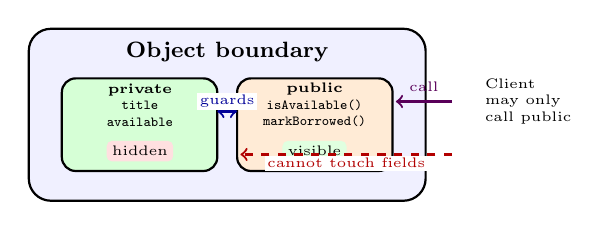
\begin{tikzpicture}[scale=0.84, every node/.style={font=\scriptsize}]
\draw[thick,fill=blue!6,rounded corners=8pt] (-3.0,-1.3) rectangle (3.0,1.3);
\node[font=\footnotesize\bfseries] at (0,0.95) {Object boundary};
\draw[thick,fill=green!16,rounded corners=5pt] (-2.5,-0.85) rectangle (-0.15,0.55);
\node[font=\tiny,align=center] at (-1.32,0.15) {\textbf{private}\\\texttt{title}\\\texttt{available}};
\node[font=\tiny,align=center,fill=red!12,rounded corners=2pt,inner sep=2pt] at (-1.32,-0.55) {hidden};
\draw[thick,fill=orange!16,rounded corners=5pt] (0.15,-0.85) rectangle (2.5,0.55);
\node[font=\tiny,align=center] at (1.32,0.15) {\textbf{public}\\\texttt{isAvailable()}\\\texttt{markBorrowed()}};
\node[font=\tiny,align=center,fill=green!12,rounded corners=2pt,inner sep=2pt] at (1.32,-0.55) {visible};
\draw[<->,thick,blue!60!black] (-0.15,0.05) -- (0.15,0.05) node[midway,above,font=\tiny,fill=white,inner sep=1pt] {guards};
\draw[->,thick,violet!70!black] (3.4,0.2) -- (2.55,0.2) node[midway,above,font=\tiny] {call};
\node[font=\tiny,align=left] at (4.55,0.2) {Client\\may only\\call public};
\draw[->,thick,red!70!black,dashed] (3.4,-0.6) -- (0.2,-0.6) node[midway,below,font=\tiny,fill=white,inner sep=1pt] {cannot touch fields};
\end{tikzpicture}
\caption{Encapsulation: private state is hidden behind a public interface. All state changes go through methods that can enforce invariants.}
\label{fig:encapsulation-wall}
\end{figure}

\section{Encapsulation and Access Control}
\label{sec:encapsulation}
\emph{Encapsulation} bundles data and the methods that maintain it, and hides the data. Java enforces this with visibility:

\begin{center}
\begin{tabular}{lcccc}
\toprule
Modifier & class & package & subclass & world \\
\midrule
\texttt{private} & \checkmark & & & \\
package (default) & \checkmark & \checkmark & & \\
\texttt{protected} & \checkmark & \checkmark & \checkmark & \\
\texttt{public} & \checkmark & \checkmark & \checkmark & \checkmark \\
\bottomrule
\end{tabular}
\end{center}

Rule of thumb: make fields \texttt{private} by default; expose behaviour, not data. Provide getters only when callers truly need the information, and prefer telling objects what to do over asking for data and deciding externally (``Tell, Don't Ask'').

\subsection{Static vs.\ Instance}
\texttt{static} members belong to the \emph{class} (one copy): constants, factories, counters of instances. Instance members belong to each \emph{object}. Confusing them is a common bug: \texttt{static int nextId} is shared; \texttt{int id} is per-object.

\subsection{Immutability and Defensive Copies}
An \emph{immutable} class has no mutators and all fields \texttt{final}---instances cannot change after construction (e.g., \texttt{String}, \texttt{LocalDate}). Immutability eliminates aliasing bugs. When a class holds a mutable field (e.g., \texttt{Date} or \texttt{List}), return defensive copies or wrap with \texttt{Collections.unmodifiableList}.

% --- TikZ 3: identity vs equality ---
\begin{figure}[h]
\centering
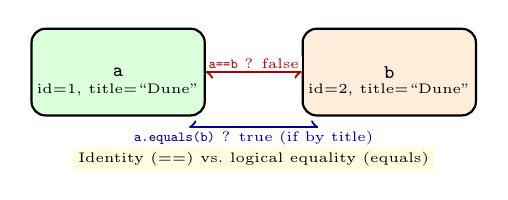
\begin{tikzpicture}[scale=0.82, every node/.style={font=\scriptsize}]
\node[draw,thick,fill=green!14,rounded corners=5pt,minimum width=2.2cm,minimum height=1.1cm] (a) at (0,0) {\texttt{a}};
\node[font=\tiny] at (0,-0.28) {id=1, title=``Dune''};
\node[draw,thick,fill=orange!14,rounded corners=5pt,minimum width=2.2cm,minimum height=1.1cm] (b) at (4.2,0) {\texttt{b}};
\node[font=\tiny] at (4.2,-0.28) {id=2, title=``Dune''};
\draw[<->,thick,red!70!black] (a) -- (b) node[midway,above,font=\tiny,fill=white,inner sep=1pt] {\texttt{a==b} ? false};
\draw[<->,thick,blue!60!black] (1.1,-0.85) -- (3.1,-0.85) node[midway,below,font=\tiny,fill=white,inner sep=1pt] {\texttt{a.equals(b)} ? true (if by title)};
\node[font=\tiny,align=center,fill=yellow!12,rounded corners=2pt,inner sep=2pt] at (2.1,-1.35) {Identity (==) vs.\ logical equality (equals)};
\end{tikzpicture}
\caption{Identity (\texttt{==}) checks same object; \texttt{equals} checks logical equivalence as defined by the class.}
\label{fig:identity-equality}
\end{figure}

\section{Identity, Equality, and String Representation}
\label{sec:identity}
Java has two equalities: \texttt{==} (same heap object) and \texttt{equals} (logical equality). Default \texttt{equals} is identity---override it when value-semantics matter, and always override \texttt{hashCode} consistently: equal objects must have equal hashes.

\begin{lstlisting}[language=Java, caption={Equality contract and toString---value semantics done right.}]
public final class Isbn {
    private final String code;
    public Isbn(String code) { this.code = code; }
    @Override public boolean equals(Object o) {
        if (this == o) return true;
        if (!(o instanceof Isbn)) return false;
        return code.equals(((Isbn)o).code);
    }
    @Override public int hashCode() { return code.hashCode(); }
    @Override public String toString() { return "Isbn[" + code + "]"; }
}
\end{lstlisting}

\begin{remark}[Common pitfall]
Storing mutable objects in \texttt{HashSet}/\texttt{HashMap} and then mutating fields that affect \texttt{hashCode} corrupts the collection. Prefer immutable keys.
\end{remark}

\section{Constructors, Overloading, and Object Lifecycle}
\label{sec:constructors-lifecycle}
A constructor's job is to establish the invariant from birth. If construction can fail, fail fast with an exception---never create a ``zombie'' object that is half-initialised.

\paragraph{Constructor chaining.} One constructor should do the work; others delegate via \texttt{this(...)} so validation lives in one place.

\begin{lstlisting}[language=Java, caption={Constructor chaining---single validation point.}]
public class Member {
    private final String id;
    private final String name;
    private final int maxLoans;
    public Member(String id, String name){ this(id, name, 5); }
    public Member(String id, String name, int maxLoans){
        if (id==null||name==null) throw new IllegalArgumentException("id/name required");
        if (maxLoans<1||maxLoans>10) throw new IllegalArgumentException("maxLoans 1..10");
        this.id=id; this.name=name; this.maxLoans=maxLoans;
    }
}
\end{lstlisting}

\paragraph{Overloading vs.\ overriding (preview of Ch.~3).} Overloading is same name, different parameters, resolved at compile time. It is convenient for constructors and utility methods but can surprise with autoboxing/null. Overriding (runtime, via inheritance) is covered fully in Ch.~3.

\paragraph{Lifecycle: creation $\to$ use $\to$ GC.} After \texttt{new}, the object is reachable while referenced; when unreachable it becomes eligible for garbage collection. No explicit \texttt{free} is needed. Reachability explains memory leaks: a forgotten observer list entry keeps an object alive forever---see Ch.~6.

\subsection{Records and Compact Value Types (Java 16+)}
For immutable data carriers, \texttt{record} generates constructor, accessors, \texttt{equals}/\texttt{hashCode}/\texttt{toString} automatically.
Ideal for value objects like \texttt{Isbn}, \texttt{Money}, \texttt{IsbnRange}. Use a class when you need mutability or invariant enforcement beyond the canonical constructor.

\subsection{Common Pitfalls and How Tests Catch Them}
\begin{itemize}[itemsep=0.25em]
    \item \emph{Exposing mutable internals.} Return an unmodifiable view (e.g., \texttt{Collections.unmodifiableList(books)}) or a copy; otherwise \texttt{library.getBooks().clear()} destroys state. A test that mutates the returned list and checks the library still has its books catches this.
    \item \emph{Inconsistent equals/hashCode.} Two equal \texttt{Isbn} objects landing in different hash buckets breaks \texttt{HashSet} lookup. Test: add equal objects, assert \texttt{set.size()==1} and \texttt{set.contains(copy)}.
    \item \emph{Forgetting defensive copies of Date/List.} Caller mutates the object after passing it in. Fix: copy on entry (\texttt{this.dueDate = LocalDate.from(dueDate)}) and on exit; \texttt{LocalDate} is already immutable, which is why modern Java prefers it over \texttt{Date}.
\end{itemize}

\begin{lstlisting}[language=Java, caption={Defensive copy for a mutable field (contrast with immutable LocalDate).}]
class Loan {
    private final LocalDate dueDate; // immutable -- no copy needed
    private final List<String> notes; // mutable -- must copy
    Loan(LocalDate dueDate, List<String> notes){
        this.dueDate = dueDate; // LocalDate is immutable
        this.notes = List.copyOf(notes); // defensive copy + unmodifiable
    }
    List<String> getNotes(){ return notes; } // already unmodifiable
}
\end{lstlisting}

\section{Chapter Notes}
Encapsulation is Parnas (1972); ``Tell, Don't Ask'' is Cunningham. Effective Java (Bloch) Ch.~4 covers access control, immutability, and the equals/hashCode contract. Java's package-private default is a deliberate middle ground between \texttt{private} and \texttt{public}.

\section{Exercises}
\label{sec:ch02-exercises}
\begin{enumerate}[label=E2.\arabic*, leftmargin=*, itemsep=0.8em]
    \item \textbf{Encapsulation audit.} A \texttt{BankAccount} exposes \texttt{public double balance}. Give a concrete failure this allows, then redesign with \texttt{private} + methods \texttt{deposit}, \texttt{withdraw} that preserve \texttt{balance $\ge$ 0} and explain how coupling drops.
    \item \textbf{Constructor invariants.} Write a \texttt{Member} class with \texttt{maxLoans} invariant $1 \le \texttt{maxLoans} \le 10$. Show constructor validation, a getter, and why no setter is needed. What test would catch a missing check?
    \item \textbf{Static vs.\ instance.} A student puts \texttt{private String title} as \texttt{static} in \texttt{Book}. Describe the observable failure with two \texttt{Book} instances and fix it. When \emph{should} a field be \texttt{static}?
    \item \textbf{Identity vs.\ equality.} Two \texttt{Isbn("978-0-06-025492-6")} objects: compare \texttt{==} and \texttt{equals}. Explain why \texttt{hashCode} must be overridden and give a failing \texttt{HashSet} scenario if it is not.
    \item \textbf{Defensive copies.} \texttt{Library} holds \texttt{private List<Book> books} and returns it directly. Show how a caller can break the invariant, then fix with either a copy or unmodifiable view and discuss trade-offs.
\end{enumerate}
% End of Chapter 2
